\documentclass[10pts]{beamer}
\usepackage{multicol}
\usepackage[shortlabels]{enumitem}
\usepackage{graphicx}
\usepackage{comment}
\usepackage{amsmath}

\usetheme[progressbar = frametitle]{metropolis}
\setbeamertemplate{frame numbering}[fraction]
\useoutertheme{metropolis}
\useinnertheme{metropolis}
\usefonttheme{metropolis}
\usecolortheme{spruce}
\setbeamercolor{background canvas}{bg = white}

\definecolor{ashgrey}{rgb}{.52,.52,.51}
\usecolortheme[named=ashgrey]{structure}
\graphicspath{{../images/}}      


\title[Matrix chain Problem]{Flop count vs. Efficiency}
\author{Edilbert Christhuraj and Sadulla Aghayev}
\institute{RWTH Aachen}
\date{February 2, 2018}

\begin{document}
   \metroset{block=fill}
   
   \begin{frame}
   	\titlepage
   \end{frame}
	 
	    \begin{frame}[t]{Problem Statement} \vspace{10pt}
	    
	    \textit{"In the design of a numerical algorithms, one typically tends to minimize the number of floating point operations, with the intention of minimizing the execution time. The underlying assumption, which unfortunately does not hold in practice, is that all flops cost the same.\\ \vspace{2pt}
	    The project is an investigation of the difference between flop count and execution time, plus a study of sensitivity to perturbations"}.\vspace{20pt}
	
     	\hspace{160pt} \textbf{Prof. Dr. Paolo Bientinesi}\\
     		\hspace{86pt} Hight Performance and Automatic Computing\\
		
		\end{frame}
	   	
	   	 \begin{frame}[t]{Our goals }\vspace{5pt}
	   	 	\section{We need to...}
	   	 	\begin{enumerate}[(\roman{*})]
	   	 		\item investigate difference between flop count and execution time
	   	 		\item verify the statement - "All flops do not cost the same"
	   	 		\item carry out a perturbation analysis
	   	 	\end{enumerate} 
	   	 	\section{Additional requirement} 
	   	 	 use an optimized BLAS library function to perform computations    
	   	 \end{frame}
	   	 
	   
	    \begin{frame}[t]{Recall}
	        Matrix multiplication is associative but not always commutative\\
	    	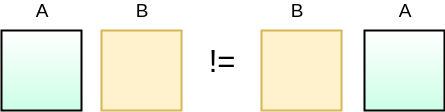
\includegraphics[scale =0.3]{square_mat_commutation.png}\\
	    	Dimensions must agree\\
	    	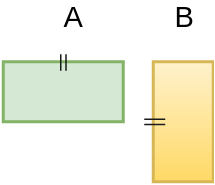
\includegraphics[scale =0.3]{matrix_commutation.png}\\
	    	 Matrix chain multiplication \\ 
	    	 	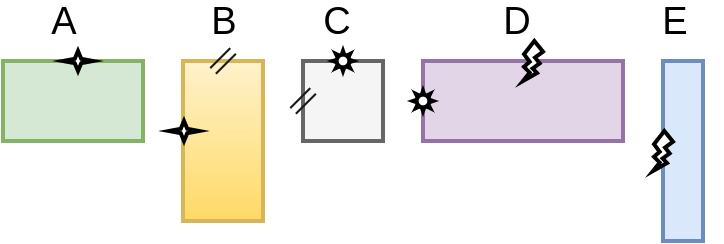
\includegraphics[scale =0.3]{chain_matrix.png}
	    \end{frame}
	    
	    
	   	\begin{frame}{A simple 3 matrices chain}
	   	     \begin{center}
	   	     	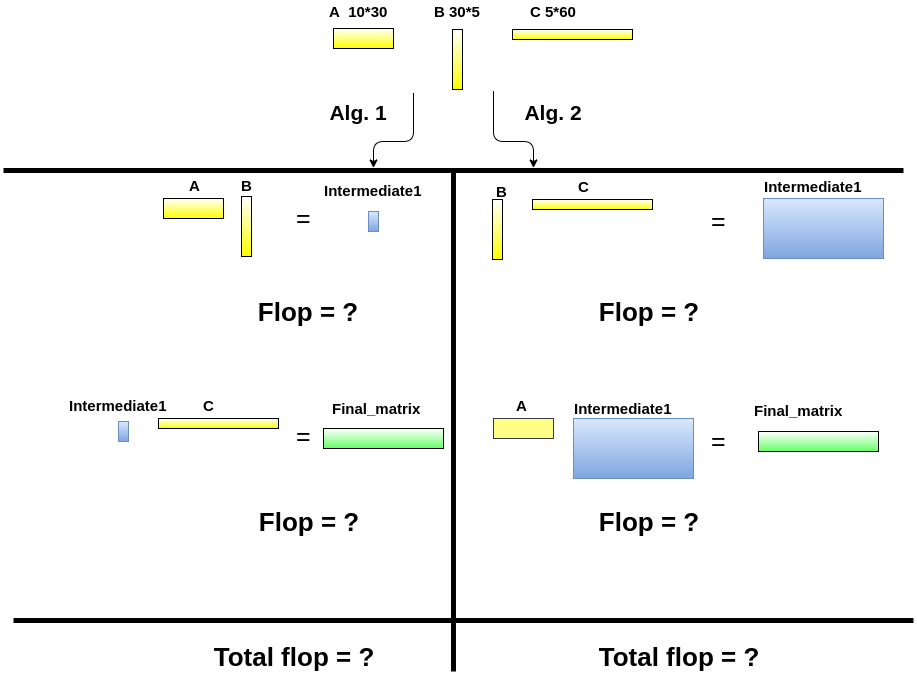
\includegraphics[scale =0.3]{3mat_1.png}
	   	     \end{center}
	   	\end{frame}
	   	
	   	  
	   	  \begin{frame}{FLOP calculation}
	   	  	\begin{center}
	   	  	 FLOP - Floating Point Operation \vspace{20pt}	
	   	  
	   	 
	   	  \begin{columns}
	           \column{0.5\textwidth}   	 
	   	        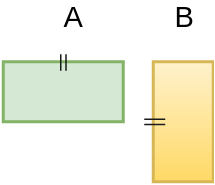
\includegraphics[scale =0.3]{matrix_commutation.png}
	   	        
	   	        A $(m*n)$ and B $(n*k)$
	   	        
	   	       
	   	 
	   	      \column{0.5\textwidth}
	   	          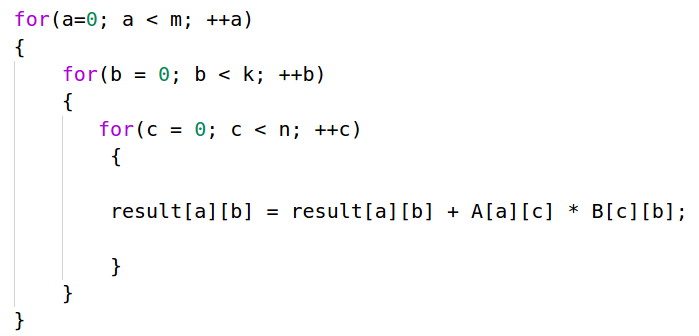
\includegraphics[scale =0.24]{tripple_loop.png}
	   	          
	   	         
	   	  \end{columns}
	   	  \vspace{15pt}
	   	   \textcolor{red}{Flop = $2*m*n*k$}
	   	   
	   	   
	   	   Example:  A $(10*20)$ and B $(20*4)$\\
	   	   $Flop = 2*10*20*4 = 1600$ 
	   	  	
	   	  	\end{center}
	   	  \end{frame}
	   	
	   	\begin{frame}{A simple 3 matrices chain}
	   		 \begin{center}
	   			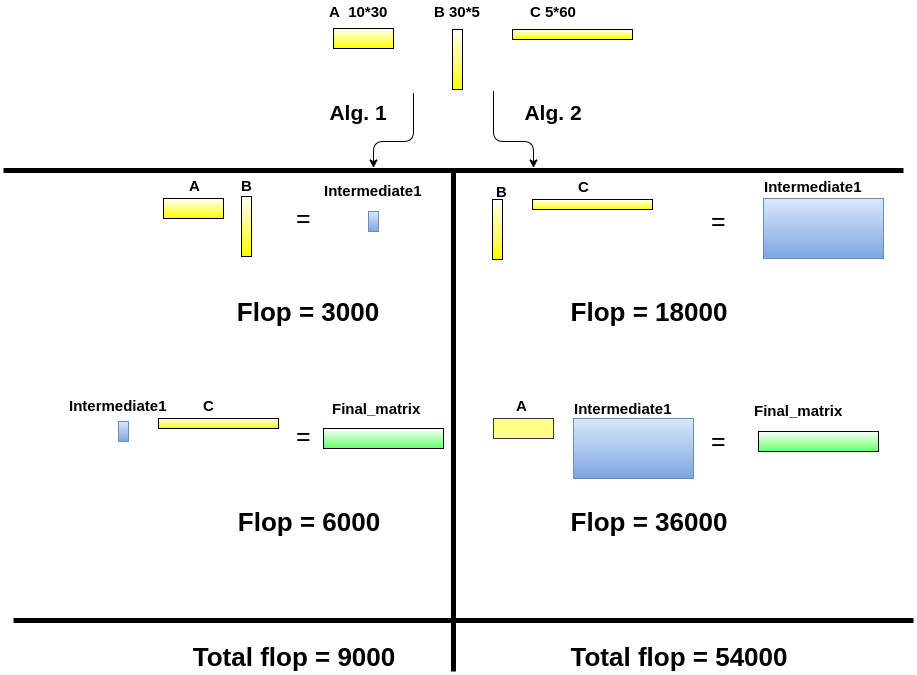
\includegraphics[scale =0.3]{3mat_1_full.png}
	   		 \end{center}
	   	\end{frame}
		
	   	\begin{frame}{A simple 3 matrices chain}
	   	     \begin{columns}
		   		 \column{.7\textwidth}
		   	     \begin{center}
	   	     		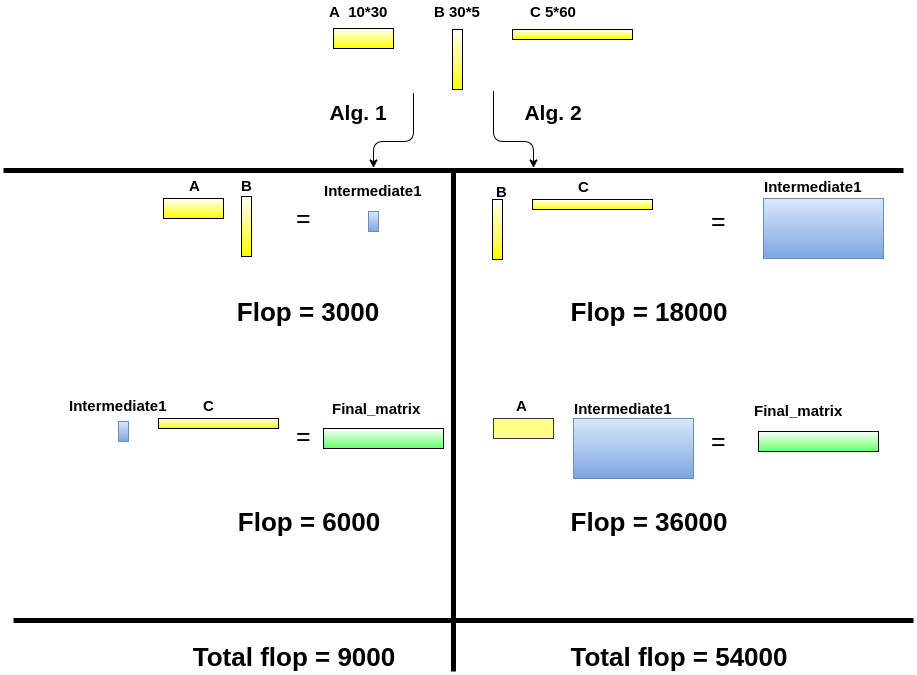
\includegraphics[width=70mm,scale =0.3]{3mat_1_full.png}
		   	     \end{center}
	   	     
		   		\column{0.5\textwidth}
		   		 $(A*B)*C$  $ =$ $A*(B*C)$\\
		   		 Flop$(Alg. 1)$ $\neq$ Flop$(Alg. 2)$\\
		   		 \begin{center}
		   		  and  execution time?
		   		 \end{center}
		   	\end{columns}	
	   	\end{frame} 
	   	
	   	\begin{frame}[t]{Catalan number and Parenthesization}
	   		\begin{center}
              	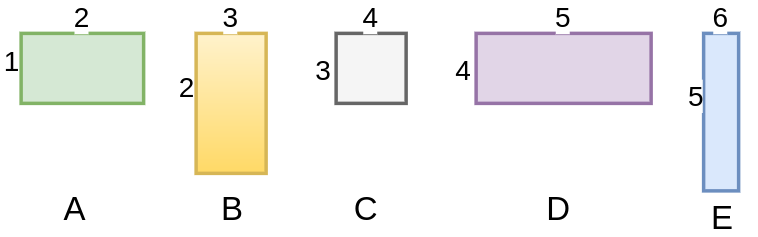
\includegraphics[scale =0.2]{chain_matrix_numero.png}
	   		\end{center}
	   		
	   	
	   		\begin{center}
	   		possibility-1	(((A*B)*C)*D)*E \hspace{80pt}
	   			  
	   		possibility-2	A*(B*(C*(D*E))) \hspace{80pt}
	   				 			
	   		\end{center}
	   		 	how many possibilities in total?\\
	   	
	   		   $P_n$ parenthesization: $P_n = C_{n-1}$\\\vspace{3pt}
	           $n^{th}$ Catalan number : $C_n = \frac{1}{n+1} \binom{2n}{n}$ \\
	     
	   	\begin{center}
	   	\begin{tabular}{c c c c c c c c c c}
	   		   n  & 2 & 3 & 4 & \textcolor{red}{5} & 6 & 7 & 8 & 9\\ 
	   		$P_n$ & 1 & 2 & 5 & \textcolor{red}{14} & 42 & 132 & 429 & 1430
	   	\end{tabular} 
	   	\end{center}
	   		
	   		
	   	\end{frame} 	
	 
	 	\begin{frame}[t]{5 Matrices chain}
	 		\begin{center}
	 			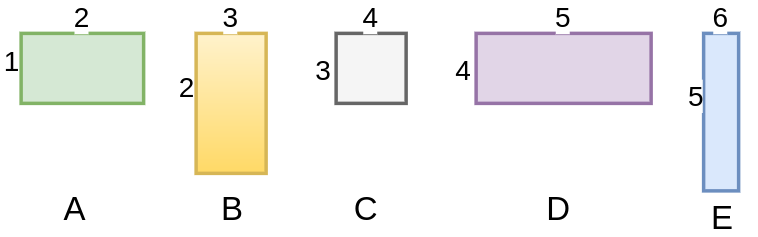
\includegraphics[scale =0.2]{chain_matrix_numero.png}
	 		\end{center}
	 		
	 		   	\begin{center}
	 		   	
	 		   	\textcolor{red}{Alg.-0} (((A*B)*C)*D)*E  \hspace{30pt}\textcolor{red}{Alg.-5} A*(B*((C*D)*E))\\
	 		   	
	 		   	\textcolor{red}{Alg.-1} (A*(B*(C*D)))*E \hspace{30pt}\textcolor{red}{Alg.-6} A*((B*(C*D))*E) \\
	 		   	\textcolor{red}{Alg.-2} A*(B*(C*(D*E))) \hspace{30pt}\textcolor{red}{Alg.-7} (A*B)*(C*(D*E))\\
	 		   	\textcolor{red}{Alg.-3} A*(((B*C)*D)*E) \hspace{30pt}\textcolor{red}{Alg.-8} (A*B)*((C*D)*E) \\
	 		   	\textcolor{red}{Alg.-4} A*((B*C)*(D*E)) \hspace{30pt}\textcolor{red}{Alg.-9} ((A*B)*C)*(D*E)\\
	 		   	 
	 		   	
	 		   	
	 		   	
	 		   
	 		   	\textcolor{red}{Alg.-10} (A*(B*C))*(D*E)\\
	 		   	\textcolor{red}{Alg.-11} ((A*(B*C))*D)*E\\
	 		   	\textcolor{red}{Alg.-12} (A*((B*C)*D))*E\\
	 		   	\textcolor{red}{Alg.-13} ((A*B)*(C*D))*E\\
	 		   	
	 			   	 			
	 			\end{center}
	 			
	 	\end{frame} 	
	 	
	 	
	 	
	 	\begin{frame}{5 Matrices chain}
	 	    \begin{center}
	 		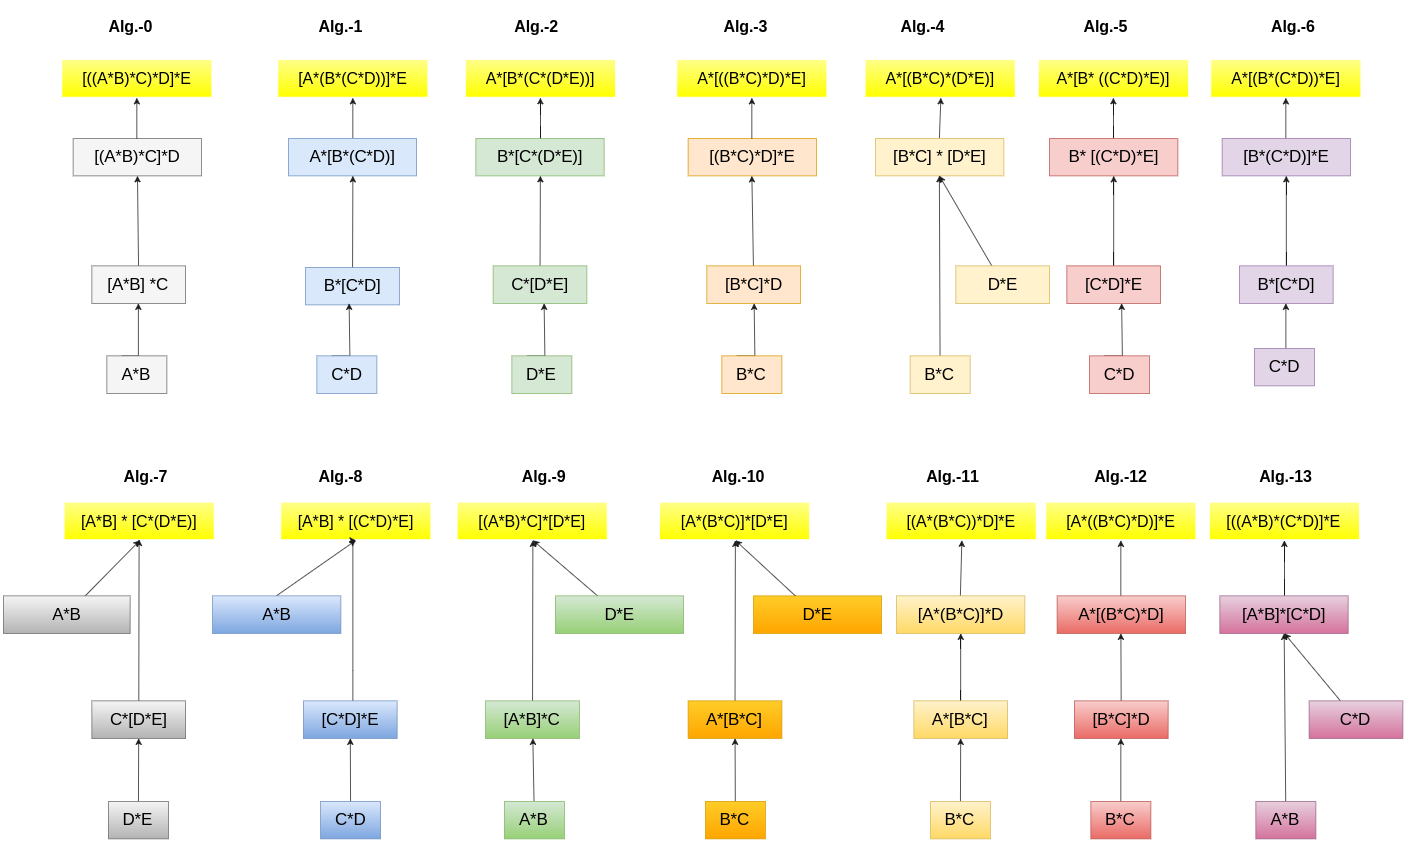
\includegraphics[scale =0.23]{5mat_color_black_Arrow.png}
	 		\end{center}
	 	\end{frame}
	 	
	 	%%\begin{frame}{5 Matrices chain}
	 	%%	\begin{center} Alg. 4\\
	 	%%	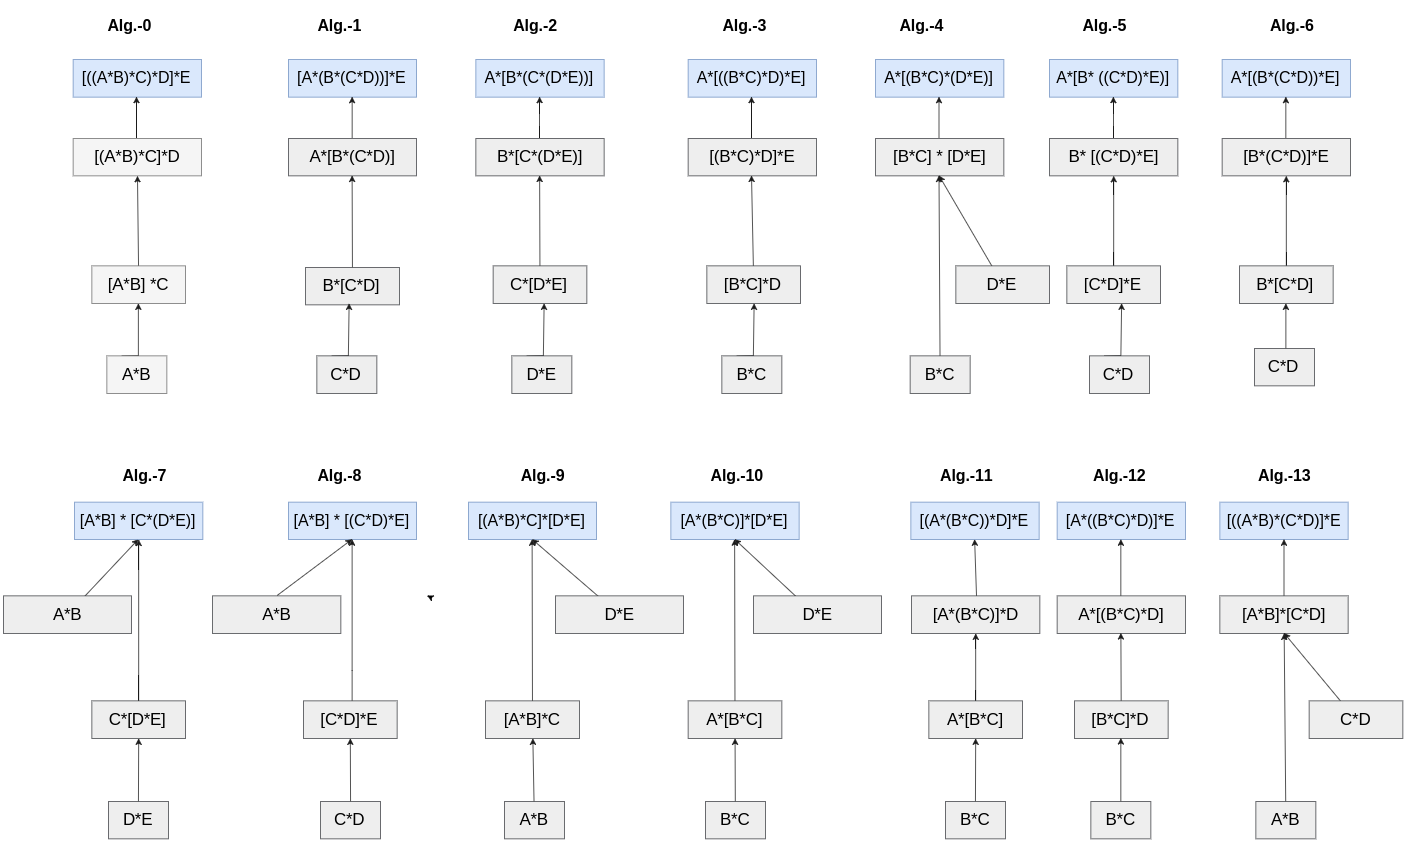
\includegraphics[scale =0.23]{5mat_gray.png}
	 	%%	\end{center}
	 	%%\end{frame} 
	 
	 \begin{frame}[t]{Quantities that we are interested in are :}
	 	\begin{center}
	 		\begin{enumerate}[(\roman{*})]
	 		\item \textbf{Flop} - How many floating point operations does each algorithm perform? \\
	 		
	 			\textcolor{red}{min\textunderscore flop\textunderscore alg}   - Algorithm which performs minimum flop\\
	 		
	 		\item \textbf{Execution time (in Seconds)} - How much time does each algorithm take to execute?
	 		
	 			\textcolor{blue}{min\textunderscore time\textunderscore alg}   - Algorithm which takes minimum time to execute\\
	 		\item $\textbf{Deviation (in \%)} = \frac{t_{min \textunderscore flop \textunderscore alg}-t_{min\textunderscore time \textunderscore alg}}{t_{min \textunderscore time \textunderscore alg}} *100$ \\
	 		How much percentage is the "$min\textunderscore time\textunderscore alg$" faster than the "$min\textunderscore flop\textunderscore alg$" ? \\
	 	
	 		\textcolor{red}{$t_{min \textunderscore flop \textunderscore alg}$} - time for minimum flop algorithm\\
	 		\textcolor{blue}{$t_{min\textunderscore time \textunderscore alg}$}  -  time for minimum time algorithm
	 		\end{enumerate}
	 	\end{center}
	 	
	 	
	 		
	 		
	 \end{frame}
	 
	 
	 
	 
	 	\begin{frame}{Pseudo algorithm}
	 		\begin{columns}
	 			\column{.4\textwidth}
	 		
	 			main \{ \\
	 			    \hspace{30pt}Timer start\\
	 				 \hspace{65pt}Alg. 0\\
	 				\hspace{30pt}Timer finish\\
	 				
	 				  \hspace{30pt}Timer start\\
	 				  \hspace{65pt}Alg. 1\\
	 				  \hspace{30pt}Timer finish\\
	 			    	\hspace{30pt} ...\\	 				 
	 				  \hspace{30pt}Timer start\\
	 				  \hspace{65pt}Alg. 13\\
	 				  \hspace{30pt}Timer finish\\
	 				
	                  
	                  \hspace{28pt}  \} 	\\		
	 		
	 			
	 			\column{0.6\textwidth}
	 			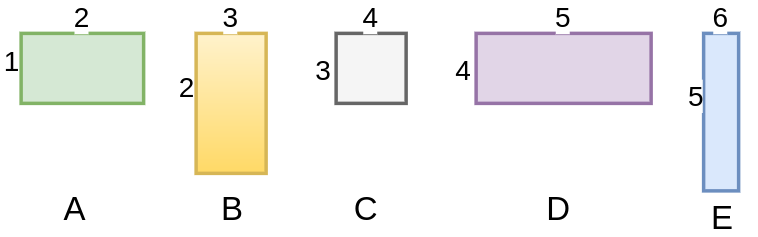
\includegraphics[scale =0.18]{chain_matrix_numero.png}
	 			
	 			Input  : 
	 			Matrix sizes$[1,2,3,4,5,6]$\\ 
	 			output :\\
	 				\begin{tabular}{ c c }
	 				 time\textunderscore 0 & flop\textunderscore 0 \\ 
	 				 time\textunderscore 1 & flop\textunderscore 1 \\ 
	 				 time\textunderscore 2 & flop\textunderscore 2 \\ 
	 				 . & .\\
	 			     . & .\\
	 				 time\textunderscore 12 & flop\textunderscore 12 \\
	 				 time\textunderscore 13 & flop\textunderscore 13 
	 				\end{tabular}\\
	 		   % Min\textunderscore flop\textunderscore alg
	 			%Min\textunderscore flop\textunderscore alg
	 			Deviation\\
	 		
	 		
	 		\end{columns}	
	 	\end{frame} 
	 
	      \begin{frame}{Additional information}
	      	
	      	
	      	\begin{block}{OpenBLAS}
	      		\begin{enumerate}[(\roman{*})]
	      			\item	OpenBLAS is an optimized BLAS library based on GotoBLAS2 
	      			\item version - 0.2.20\\
	      			\item cblas\textunderscore dgemm(.....)   	
	      		\end{enumerate}
	      	\end{block}
	      	
	      	\begin{block}{Hardware details}
	      		\begin{enumerate}[(\roman{*})]
	      			\item RWTH Clutser - MPI\textunderscore S
	      			\item https://doc.itc.rwth-aachen.de/display/CC/Hardware+of+the+RWTH+Compute
	      			\item tested only on one node 	
	      		\end{enumerate}
	      	\end{block} 
	      	
	      	\begin{block}{Programming environment}
	      		implementation in C and gcc compiler v4.0.2	
	      	\end{block} 
	      	
	      \end{frame}
	    
	      
	      \begin{frame}{Test case}
	      	\begin{center}
	      		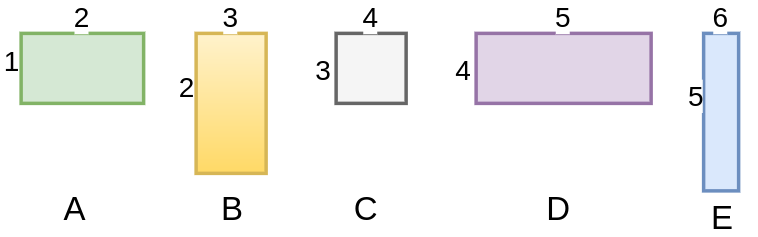
\includegraphics[scale =0.3]{chain_matrix_numero.png}\\
	      		\vspace{20pt}
	      			$1^{st}$ Chain   130 700 383 1340 193 900 \\
	      			\vspace{10pt}
	      			$2^{nd}$ Chain   376 561 477 532 425 590 
	      	\end{center}
	      
	      	
	      \end{frame}
	  
	   \begin{frame}{$1^{st}$ Chain 130 700 383 1340 193 900 \hspace{75pt}   Sample-1  }
	   	\begin{columns}
	   		\column{0.65\textwidth}
	   		
	   		\begin{tabular}{c | c | c}
	   			\textbf{Algorithm}  & \textbf{Time} (Seconds) & \textbf{Flop}\\		
	   			0	&   0.051306	&	\textcolor{red}{315,546,400}\\
	   			1	&	0.065909 	&	381,877,520\\
	   			2 	&	0.247766 	&	2,035,692,000\\
	   			3 	&	0.180365 	&	1,487,556,000 \\
	   			4 	&	0.361984 	&	3,036,224,000\\
	   			5 	&	0.118680 	&	977,537,120\\
	   			6	&    0.088250 	&	708,569,520\\
	   			7 	&	0.185151 	&	1,548,640,000\\
	   			8 	&	0.061688 	&	490,485,120\\
	   			9 	&	0.122389 	&	982,219,200\\
	   			10 	&	0.215232 	&	1,741,464,000\\
	   			11 	&	0.131261 	&	1,074,791,200\\
	   			12 	&	0.140059 	&	1,160,864,000\\
	   			13 	&	\textcolor{blue}{0.042321} 	&	332,189,860	
	   			
	   		\end{tabular}
	   		
	   		
	   		\column{0.25\textwidth}
	   		\textcolor{red}{min\textunderscore flop\textunderscore alg-0}
	   		\textcolor{blue}{min\textunderscore time\textunderscore alg-13}
	   		\textcolor{black}{Deviation-21.2\%}
	   	\end{columns}
	   \end{frame} 
	   
	   
	  
	   
	   %\begin{frame}{$1^{st}$Chain 130 700 383 1340 193 900  \hspace{75pt}   Sample-1 }
	   	%	\begin{center}
	   	%		\textcolor{red}{Alg.0} (((A*B)*C)*D)*E   performs minimum number of flop\\
	   	%		\textcolor{blue}{Alg.13} ((A*B)*(C*D))*E  is the fastest in terms of execution time\\
	   	%	\end{center}
	   		
	   %\end{frame}
	  
	  
	 \begin{frame}{$2^{nd}$ Chain 376 561 477 532 425 590 \hspace{75pt}   Sample-1 }
	 	\begin{columns}
	 		\column{0.65\textwidth}
	 		
	 		\begin{tabular}{c | c | c}
	 			\textbf{Algorithm}  & \textbf{Time} (Seconds) & \textbf{Flop}\\		
	 			0 & 0.101891 &\textcolor{red}{750,654,672}\\ 		
	 			1 &	0.099232 &	811,016,450 \\	
	 			2 &	0.140206 &	1,130,908,460 \\		
	 			3 &	0.130707 &	1,068,653,388\\
	 			4 &	0.139825 &	1,152,599,048 \\		
	 			5 &	0.126232 &	1,019,583,840	\\	
	 			6 &	0.121548 &	973,402,830 	\\	
	 			7 &	0.121522 &	979,107,824	\\	
	 			8 &	0.110458 &	867,783,204	\\	
	 			9 &	0.112590 &	894,899,232 	\\	
	 			10 &	0.124695 &	1,011,994,872 \\		
	 			11 &	0.106382 &	867,750,312 	\\	
	 			12 &	0.112451 &	906,267,008 	\\	
	 			13 &    \textcolor{blue}{0.093955} &757,945,544 		
	 			
	 		\end{tabular}
	 		
	 		
	 		\column{0.25\textwidth}
	 		\textcolor{red}{min\textunderscore flop\textunderscore alg-0}
	 		\textcolor{blue}{min\textunderscore time\textunderscore alg-13}
	 		\textcolor{black}{Deviation-8.44\%}
	 	\end{columns}
	 \end{frame} 
	   
	   
	   
	  % \begin{frame}{$2^{nd}$ Chain 376 561 477 532 425 590 }
	  %	\begin{center}
	  %		\textcolor{red}{Alg.0} (((A*B)*C)*D)*E   performs minimum number of flop\\
	  %		\textcolor{blue}{Alg.13} ((A*B)*(C*D))*E  is the fastest in terms of execution time\\
	  %	\end{center}
	   %\end{frame}
	   
	   
	   \begin{frame}{All flops do not cost the same }
	   	\begin{center}
	   		\begin{tabular}{c c c }
	   			\textbf{Matrix} & \textbf{Flop} & \textbf{FLOPS = $\frac{Flop}{Second}$}  \\ 
		   		 $(100*100) * (100*100)$ &  2,000,000    &  4,672,897,196\\ 
	   			 $(200*200) * (200*200)$ &  16,000,000   &  4,705,882,352\\ 
	   			 $(300*300) * (300*300)$ &  54,000,000   &  5,819,592,628\\
	   			 $(400*400) * (400*400)$ &  128,000,000  & 6,994,535,519\\
	   			 ..  &  ... & ...\\
	   			 ..  &  ...&...\\
	   			 ..  &  ...&...\\
	   			 $(1300*1300) * (1300*1300)$&  4,394,000,000&7,036,896,462\\
	   			 $(1400*1400) * (1400*1400)$&  5,488,000,000&7,109,296,363 \\
	   			 $(1500*1500) * (1500*1500)$&  6,750,000,000&7,048,975,235\\
	   			 ...& ...& ...\\
	   			 $(3000*3000) * (3000*3000)$&  54,000,000,000&7,404,131,916\\
	   		\end{tabular} 
	   	\end{center}
	   \end{frame} 
	  
	  \begin{frame}[t]{All flops do not cost the same }
	  	\begin{center}
	  	 	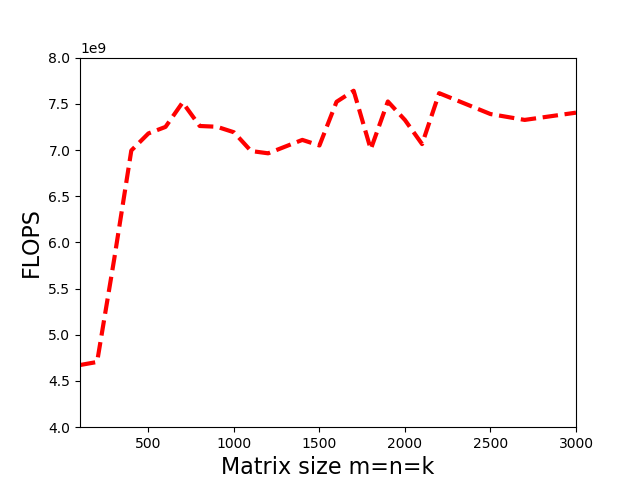
\includegraphics[scale =0.6]{benchmarkcurve.png}
	  	\end{center}
	  \end{frame} 
	  
	  
	  
	  
	   \begin{frame}[t]{Perturbation analysis }
	   
	
	    \begin{enumerate}[(\roman{*})]
	     \item \textbf{Problem} \\
	    Some of the quantities that we are interested in, such as execution times and deviation are not reproducible
	    \end{enumerate}
	     
	    
	 
	   \end{frame} 
	   
	   
	   
	    \begin{frame}{$1^{st}$ Chain 130 700 383 1340 193 900 \hspace{75pt}   Sample-1  }
	    	\begin{columns}
	    		\column{0.65\textwidth}
	    		
	    		\begin{tabular}{c | c | c}
	    			\textbf{Algorithm}  & \textbf{Time} (Seconds) & \textbf{Flop}\\		
	    			0	&   0.051306	&	\textcolor{red}{315,546,400}\\
	    			1	&	0.065909 	&	381,877,520\\
	    			2 	&	0.247766 	&	2,035,692,000\\
	    			3 	&	0.180365 	&	1,487,556,000 \\
	    			4 	&	0.361984 	&	3,036,224,000\\
	    			5 	&	0.118680 	&	977,537,120\\
	    			6	&    0.088250 	&	708,569,520\\
	    			7 	&	0.185151 	&	1,548,640,000\\
	    			8 	&	0.061688 	&	490,485,120\\
	    			9 	&	0.122389 	&	982,219,200\\
	    			10 	&	0.215232 	&	1,741,464,000\\
	    			11 	&	0.131261 	&	1,074,791,200\\
	    			12 	&	0.140059 	&	1,160,864,000\\
	    			13 	&	\textcolor{blue}{0.042321} 	&	332189860	
	    			
	    		\end{tabular}
	    		
	    		
	    		\column{0.25\textwidth}
	    		\textcolor{red}{min\textunderscore flop\textunderscore alg-0}
	    		\textcolor{blue}{min\textunderscore time\textunderscore alg-13}
	    		\textcolor{black}{Deviation-21.2\%}
	    	\end{columns}
	    \end{frame} 
	    \begin{frame}{$1^{st}$ Chain 130 700 383 1340 193 900 \hspace{75pt}   Sample-2}
	    	\begin{columns}
	    		\column{0.65\textwidth}
	    		
	    		\begin{tabular}{c | c | c}
	    			\textbf{Algorithm}  & \textbf{Time} (Seconds) & \textbf{Flop}\\		
	    			0 	&	\textcolor{blue}{0.042322} 	&	\textcolor{red}{315,546,400} \\			
	    			1 	&	0.054053 	&	381,877,520 	\\	
	    			2 	&	0.255563 	&	2,035,692,000 	\\	
	    			3 	&	0.187326 	&	1,487,556,000 	\\		
	    			4 	&	0.381132 	&	3,036,224,000 	\\		
	    			5 	&	0.120140 	&	977,537,120 	\\		
	    			6 	&	0.087574 	&	708,569,520 	\\		
	    			7 	&	0.189211 	&	1,548,640,000 	\\		
	    			8 	&	0.061826 	&	490,485,120 	\\		
	    			9 	&	0.151340 	&	982,219,200 	\\		
	    			10 	&	0.274111 	&	1,741,464,000 	\\		
	    			11 	&	0.178278 	&	1,074,791,200 	\\		
	    			12 	&	0.181404 	&	1,160,864,000 	\\		
	    			13 	&	0.045157 	&	332,189,860	\\
	    			
	    		\end{tabular}
	    		
	    		
	    		\column{0.25\textwidth}
	    		\textcolor{red}{min\textunderscore flop\textunderscore alg-0}
	    		\textcolor{blue}{min\textunderscore time\textunderscore alg-0}
	    		\textcolor{black}{Deviation-0.0\%}
	    	\end{columns}
	    \end{frame} 
	    
	    \begin{frame}{$1^{st}$ Chain 130 700 383 1340 193 900 \hspace{75pt}   Sample-3}
	    	\begin{columns}
	    		\column{0.65\textwidth}
	    		
	    		\begin{tabular}{c | c | c}
	    			\textbf{Algorithm}  & \textbf{Time} (Seconds) & \textbf{Flop}\\		
	    			0 	&	0.055871 	&	\textcolor{red}{315,546,400} 	\\		
	    			1 	&	0.056499 	&	381,877,520 	\\		
	    			2 	&	0.261406 	&	2,035,692,000 	\\		
	    			3 	&	0.206040 	&	1,487,556,000	\\		
	    			4 	&	0.387012 	&	3,036,224,000	\\		
	    			5 	&	0.131321 	&	977,537,120 	\\		
	    			6 	&	0.092505 	&	708,569,520 	\\		
	    			7 	&	0.196337 	&	1,548,640,000 	\\		
	    			8 	&	0.066044 	&	490,485,120 	\\		
	    			9 	&	0.128545 	&	982,219,200	\\		
	    			10 	&	0.226485 	&	1,741,464,000 	\\		
	    			11 	&	0.137919 	&	1,074,791,200	\\		
	    			12 	&	0.146254 	&	1,160,864,000 	\\		
	    			13 	&	\textcolor{blue}{0.044547} 	&	332,189,860 \\
	    			
	    		\end{tabular}
	    		
	    		
	    		\column{0.25\textwidth}
	    		\textcolor{red}{min\textunderscore flop\textunderscore alg-0}
	    		\textcolor{blue}{min\textunderscore time\textunderscore alg-13}
	    		\textcolor{black}{Deviation-25.4\%}
	    	\end{columns}
	    \end{frame} 
	    
	   
	    \begin{frame}{$2^{nd}$ Chain 376 561 477 532 425 590 \hspace{75pt}   Sample-1 }
	    	\begin{columns}
	    		\column{0.65\textwidth}
	    		
	    		\begin{tabular}{c | c | c}
	    			\textbf{Algorithm}  & \textbf{Time} (Seconds) & \textbf{Flop}\\		
	    			0 &	\textcolor{blue}{0.090527} &	\textcolor{red}{750,654,672}\\ 		
	    			1 &	0.096886 &	811,016,450 \\		
	    			2 &	0.133695 &	1,130,908,460 	\\	
	    			3 &	0.126657 &	1,068,653,388 	\\	
	    			4 &	0.137426 &	1,152,599,048 	\\	
	    			5 &	0.122484 &	1,019,583,840 	\\	
	    			6 &	0.116337 &	973,402,830 	\\	
	    			7 &	0.122186 &	979,107,824 	\\	
	    			8 &	0.113717 &	867,783,204 	\\	
	    			9 &	0.109312 &	894,899,232 	\\	
	    			10 &	0.123241& 	1,011,994,872\\ 		
	    			11 & 0.105787 	&867,750,312 		\\
	    			12 &	0.110508 &	906,267,008 	\\	
	    			13 &	0.091250 &	757,945,544  	\\	
	    		\end{tabular}
	    		
	    		
	    		\column{0.25\textwidth}
	    		\textcolor{red}{min\textunderscore flop\textunderscore alg-0}
	    		\textcolor{blue}{min\textunderscore time\textunderscore alg-13}
	    		\textcolor{black}{Deviation-0.0\%}
	    	\end{columns}
	    \end{frame} 
	    \begin{frame}{$2^{nd}$ Chain 376 561 477 532 425 590 \hspace{75pt}   Sample-2 }
	    	\begin{columns}
	    		\column{0.65\textwidth}
	    		
	    		\begin{tabular}{c | c | c}
	    			\textbf{Algorithm}  & \textbf{Time} (Seconds) & \textbf{Flop}\\		
	    			0 & 0.101891 &\textcolor{red}{750,654,672}\\ 		
	    			1 &	0.099232 &	811,016,450 \\	
	    			2 &	0.140206 &	1,130,908,460 \\		
	    			3 &	0.130707 &	1,068,653,388\\
	    			4 &	0.139825 &	1,152,599,048 \\		
	    			5 &	0.126232 &	1,019,583,840	\\	
	    			6 &	0.121548 &	973,402,830 	\\	
	    			7 &	0.121522 &	979,107,824	\\	
	    			8 &	0.110458 &	867,783,204	\\	
	    			9 &	0.112590 &	894,899,232 	\\	
	    			10 &	0.124695 &	1,011,994,872 \\		
	    			11 &	0.106382 &	867,750,312 	\\	
	    			12 &	0.112451 &	906,267,008 	\\	
	    			13 &    \textcolor{blue}{0.093955} &757,945,544 		
	    			
	    		\end{tabular}
	    		
	    		
	    		\column{0.25\textwidth}
	    		\textcolor{red}{min\textunderscore flop\textunderscore alg-0}
	    		\textcolor{blue}{min\textunderscore time\textunderscore alg-13}
	    		\textcolor{black}{Deviation-8.44\%}
	    	\end{columns}
	    \end{frame} 
	    
	    
	    
	    \begin{frame}{$2^{nd}$ Chain 376 561 477 532 425 590 \hspace{75pt}   Sample-3 }
	    	\begin{columns}
	    		\column{0.65\textwidth}
	    		
	    		\begin{tabular}{c | c | c}
	    			\textbf{Algorithm}  & \textbf{Time} (Seconds) & \textbf{Flop}\\	
	    			0 &	0.102252 &	\textcolor{red}{750,654,672} 	\\	
	    			1 &	0.114649 &	811,016,450 	\\	
	    			2 &	0.145311 &	1,130,908,460 	\\	
	    			3 &	0.129112 &	1,068,653,388 	\\	
	    			4 &	0.139820 &	1,152,599,048 	\\	
	    			5 &	0.129094 &	1,019,583,840 	\\	
	    			6 &	0.120107 &	973,402,830 	\\	
	    			7 &	0.120611 &	979,107,824 	\\	
	    			8 &	0.107226 &	867,783,204 	\\	
	    			9 &	0.110580 &	894,899,232 	\\	
	    			10 &	0.123456& 	1,011,994,872 \\ 		
	    			11 	&0.105604 	&867,750,312 		 \\
	    			12 	&0.110942 	&906,267,008 		\\
	    			13 	& \textcolor{blue}{0.093701} 	&757,945,544	\\
	    			
	    		\end{tabular}
	    		
	    		
	    		\column{0.25\textwidth}
	    		\textcolor{red}{min\textunderscore flop\textunderscore alg-0}
	    		\textcolor{blue}{min\textunderscore time\textunderscore alg-13}
	    		\textcolor{black}{Deviation~9.12\%}
	    	\end{columns}
	    \end{frame} 
	    
	   
	   
	   
	   
	   
	   
	   
	   
	   
	   
	   
	   
	   
	   
	   
	  
	   \begin{frame}[t]{Perturbation analysis }
	  
	   	
	   		\begin{enumerate}[(\roman{*})]
	   			\item \textbf{Problem} \\
	   		  Some of the quantities that we are interested in, such as execution times and deviation  are not reproducible
	   	
	   	
	   	         \item \textbf{Our attempts} \\
	   	         Cache flushing, different approaches for time measurements, iterations etc.\\
	   	         \textcolor{red}{no improvement}
	   	
	              \item \textbf{Remedy} \\
	              It is the \textcolor{green}{nature of the problem}.\\
	              Execution time depends not only on inputs but also on parameters such as system temperature, power supply etc.\\ 
	              Given Problem is based on \textcolor{green}{empirical statement}, not based on any mathematical equation.  
	              
	              
	   		\end{enumerate}
	   		
	   	
	  
	   \end{frame} 
	   
	  
	   \begin{frame}{Goal of Perturbation analysis }
	   	\begin{center}
	   		\begin{tabular}{c | c |c | c}
	   		\textbf{Perturbation} & \textbf{Deviation} & \textbf{Deviation} & \textbf{Flop }\\
	   		\textbf{percentage}& \textbf{range}&\textbf{frequency}&\textbf{difference}\\
	   		
	   		+15\%	&	 		&			&\\	
	   		+10\%	&	 		&			&  \\ 
	   		+5\%	&    		&			&	\\
	   		+3\%	&    		&			&	\\
	   		+1\%	&    	&		    &	\\
	   		\textcolor{blue}{130} \textcolor{blue}{700} \textcolor{blue}{383} \textcolor{blue}{1340} \textcolor{blue}{193} \textcolor{blue}{900}	&    \textcolor{blue}{0.01-36 \%}		&	\textcolor{blue}{27\%}		&	\textcolor{blue}{16,643,460}\\
	   		-1\%	&    		&			&	\\
	   		-3\%	&    		&			&	\\
	   		-5\%	&    		&			&	\\
	   		-10\%	& 	 		&			&	\\
	   		-15\%	&	 		&			&	\\
	   		\end{tabular}
	   	\end{center}
	   \end{frame} 
	  
	
	  
	
	
	  
	  \begin{frame}{$1^{st}$ Chain \hspace{30pt} \textcolor{orange}{All elements perturbation} }
	  	\begin{tabular}{c | c |c | c}
	  		\textbf{Perturbation} & \textbf{Deviation} & \textbf{Deviation} & \textbf{Flop }\\
	  		\textbf{percentage}& \textbf{range}&\textbf{frequency}&\textbf{difference}\\
	  		
	  		+15\%	&	 0.01-29 \%		&	25\%		&	25,128,102\\
	  		+10\%	&	 3.5-15 \%		&	8\%			&   21,006,788\\
	  		+5\%	&    0.01-68 \%		&	30\%		&	19,442,328\\
	  		+3\%	&    0.01-40 \%		&	40\%		&	18,752,952\\
	  		+1\%	&    0.01-18.5\%	&	40\%	    &	16,653,820\\
	  		\textcolor{blue}{130} \textcolor{blue}{700} \textcolor{blue}{383} \textcolor{blue}{1340} \textcolor{blue}{193} \textcolor{blue}{900}	&    \textcolor{blue}{0.01-36 \%}		&	\textcolor{blue}{27\%}		&	\textcolor{blue}{16,643,460}\\
	  	   -1\%	&    0.01-21 \%		&	26\%		&	17,017,292\\
	  	   -3\%	&    0.01-42 \%		&	30\%		&	15,064,266\\
	  	   -5\%	&    0.01-80 \%		&	34\%		&	14,485,500\\
	  	   -10\%	& 	 0.01-22 \%		&	30\%		&	11,569,284\\
	  	 	-15\%	&	 0.01-18 \%		&	28\%		&	10,609,780\\
	  		
	  		
	  		
	  		
	  	
	  	\end{tabular}
	  \end{frame}
	  
	  \begin{frame}{$2^{nd}$ Chain \hspace{30pt} \textcolor{orange}{All elements perturbation}}
	  	\begin{tabular}{c | c |c | c}
	  		\textbf{Perturbation} & \textbf{Deviation} & \textbf{Deviation} & \textbf{Flop }\\
	  		\textbf{percentage}& \textbf{range}&\textbf{frequency}&\textbf{difference}\\
	  	
	  		+15\%	&	0.01-15 \%		&	46.5\%	&		10,937,920\\
	  		+10\%	&	3.5-6\%			&    48\%	&		9,576,058\\
	  		+5\%	&	0.01-67 \%		&	52.5\%	&		8,632,016\\
	  		+3\%	&	0.01-20 \%		&	43\%	&		7,916,372\\
	    	+1\%	&	0.01-19 \%		&	63\%	&		7,619,508\\
	 \textcolor{blue}{376} \textcolor{blue}{561} \textcolor{blue}{477} \textcolor{blue}{532} \textcolor{blue}{425} \textcolor{blue}{590}	&    \textcolor{blue}{0.01-22 \%}		&	\textcolor{blue}{40\%}		&	\textcolor{blue}{7,290,872}\\
	  	-1\%	&	0.01-13 \%		&	65\%	&		6,960,192\\	
	  	-3\%	&	0.01-20 \%		&	47.5\%	 &		6,89,088\\
	  	-5\%	&	0.01-73 \%		&	57\%	 &		6,083,796\\
	  	-10\%	&	0.01-34 \%		&	43\%   	 &		5,392,088\\
	  	-15\%	&	0.01-19 \%		&	40\%	 &		4,552,094\\
	  	
	  	
	  	
	  	
	  	
	  	\end{tabular}
	  \end{frame}
	  
	   \begin{frame}{$1^{st}$ Chain \hspace{30pt} \textcolor{orange}{Single element perturbation (5\%)} }
	      \begin{tabular}{c| c | c |c | c}
	   		&\textbf{Matrix} & \textbf{Deviation} & \textbf{Deviation}& \textbf{Flop }\\
	     	\%&\textbf{chain}  & \textbf{range}     &\textbf{frequency}&\textbf{difference}\\
	   	    % 130 700 383 1349 193 900 &	0.01-36 \%	&	   27\% 	&		16,643,460\\
	   	    \textcolor{green}{+}&\textcolor{green}{136} 700 383 1340 193 900 &	0.01-25 \%	&		53\%	&		8,628,408\\
	   	    \textcolor{green}{+}&130 \textcolor{green}{735} 383 1340 193 900 &	0.01-67 \%	&		33\%	&		16,643,460\\	
	   	    \textcolor{green}{+}&130 700 \textcolor{green}{402} 1340 193 900 &	0.01-24 \%	&		30\%	&		20,804,840\\	
	   	    \textcolor{green}{+}&130 700 383 \textcolor{green}{1407} 193 900 &	0.01-74 \%	&		46\%	&		16,514,686\\
	   	    \textcolor{green}{+}&130 700 383 1340 \textcolor{green}{202} 900 &	2 - 21 \%		&     	26\%	&		23,642,040\\
	   	    \textcolor{green}{+}&130 700 383 1340 193 \textcolor{green}{945} &	1 - 40 \%		&	    36\%	&		16,643,460\\
	   	   	 & \textcolor{blue}{130} \textcolor{blue}{700} \textcolor{blue}{383} \textcolor{blue}{1340} \textcolor{blue}{193} \textcolor{blue}{900} &	\textcolor{blue}{0.01-36 \%}	  &	    \textcolor{blue}{27\%}	&		\textcolor{blue}{16,643,460}\\
	   	   \textcolor{red}{-}& \textcolor{red}{123} 700 383 1340 193 900 &	0.01-50 \%	  &		23\%	&		26,414,454\\
	   	   \textcolor{red}{-}&130 \textcolor{red}{665} 383 1340 193 900 &	0.01-85 \%	  &		56\%	&		16,643,460\\	
	   	   \textcolor{red}{-}&130 700 \textcolor{red}{363} 1340 193 900 &	0.01-13 \%	  & 	43\%	&		9,263,060\\
	   	   \textcolor{red}{-}&130 700 383 \textcolor{red}{1273} 193 900 &	4 - 84 \%		  &	    30\%	&		16,772,234\\
	   	   \textcolor{red}{-}&130 700 383 1340 \textcolor{red}{183} 900 &	0.01-26\%	  &		56\%	&		 8,867,260\\
	   	   \textcolor{red}{-}&130 700 383 1340 193 \textcolor{red}{855} &	0.01-39 \%	  &	    36\%	&		16,643,460\\
	   		
	     \end{tabular}
	   \end{frame}
	   
	
	   
	   \begin{frame}{$2^{nd}$ Chain \hspace{30pt} \textcolor{orange}{Single element perturbation (5\%)}}
	   	\begin{tabular}{c|c | c |c | c}
	   		&\textbf{Matrix} & \textbf{Deviation} & \textbf{Deviation} & \textbf{Flop }\\
	   		\%&\textbf{chain}& \textbf{range}&\textbf{frequency}&\textbf{difference}\\
	   	    
	   	      \textcolor{green}{+}&\textcolor{green}{394} 561 477 532 425 590	&	0.01-11 \%	 &		23\%	&		2,686,132\\
	   	      \textcolor{green}{+}&376 	\textcolor{green}{589} 477 532 425 590	&	0.01-17 \%	 &		40\%	&		7,290,872\\	
	   	      \textcolor{green}{+}&376 561 	\textcolor{green}{500} 532 425 590	&	0.01-49 \%	 &		50\%	&		15,840,800\\	
	   	     \textcolor{green}{+} &376 561 477 	\textcolor{green}{558} 425 590	&	0.01- 5 \%	 &		23\%	&		   196,668\\
	   	     \textcolor{green}{+} &376 561 477 532 	\textcolor{green}{446} 590	&	0.01-12\%	 &		30\%	&		17,080,400\\
	   	      \textcolor{green}{+}&376 561 477 532 425 	\textcolor{green}{619}	&	0.01-16 \%	&		43\%	&		7,290,872\\
	   	      &\textcolor{blue}{376} \textcolor{blue}{561} \textcolor{blue}{477} \textcolor{blue}{532} \textcolor{blue}{425} \textcolor{blue}{590}	&	\textcolor{blue}{0.01-22 \%}	&		\textcolor{blue}{40\%}	&		\textcolor{blue}{7,290,872}\\
	   	     \textcolor{red}{-} &\textcolor{red}{357} 561 477 532 425 590	  &  	0.01-24 \%		&	26\%		&	17,822,154\\
	   	      \textcolor{red}{-} &376 	\textcolor{red}{532} 477 532 425 590	  &	    0.01-32 \%		&	41\%		&	7,290,872	\\
	   	    \textcolor{red}{-} &376 561 	\textcolor{red}{453} 532 425 590	  &	    0.01-11 \%		&	26\%		&	1,630,792	\\
	   	    \textcolor{red}{-} &376 561 477 	\textcolor{red}{505} 425 590	  &	    0.01-44 \%		&	43\%		&	14,657,930\\
	   	    \textcolor{red}{-} &376 561 477 532 	\textcolor{red}{403} 590	  &	    0.01- 9 \%		&	26\%		&	2,964,824\\
	   	    \textcolor{red}{-} &376 561 477 532 425 	\textcolor{red}{560}	  &	    0.01-31 \%		&	43\%		&	7,290,872\\
	   	      
	   		
	   	\end{tabular}
	   \end{frame}
	
	  \begin{frame}{Conclusion}
	  	\begin{enumerate}[(\roman{*})]
	  	\item we investigated the relation between flop count and execution time
	  	and we verified the statement "all flops do not cost the same". 
        
       \item we carried out a perturbation analysis and studied quantities such as Flop difference, deviation range and  deviation frequency for perturbed matrix chains. 
        \end{enumerate}  	
	  \end{frame}
	  
	  
	  \begin{frame}{References}
	  	\begin{enumerate}[(\roman{*})]
	  		\item link to OpenBLAS \hspace{30pt} \\ \url{http://www.openblas.net/}
	  		\vspace{20pt}
	  		\item link to dissertation "Performance Modeling and Prediction
	  		for Dense Linear Algebra"\hspace{30pt} \url{https://arxiv.org/pdf/1706.01341.pdf}
	  		\vspace{20pt}
	  		\item link to our source code \hspace{30pt} \\
	  		\url{https://github.com/edilbert24/Sisc-Lab/tree/master/Final_Sisc_code}
	  		
	  	\end{enumerate}  	
	  \end{frame}
	  
	  
\end{document}